\section{Sammanfattning av energiflöden: energibalanser}

De olika energiflödena är alltså från fasta energikällor, flöde genom väggarna, burspråk och 
tak, genom grunden, av solinstrålning in och strålning ut genom fönstren samt från ofrivillig 
ventilation. Den sista punkten, som orsakas av vind, utelämnas i ett första steg.

Från fasta energikällor fås alltid ett bidrag på totalt $\unit[10,5]{kW}$, se avsnitt \ref{sec:constsources}.

Ur figurerna i avsnitt \ref{sec:steadystatewall} får vi energiflödena per kvadratmeter genom de 
olika avsnitten av klimatskalet och med hjälp av areorna i tabell \ref{tbl:uvalue} fås det totala 
energiutflödet genom husets hela klimatskal.

Flödet genom grunden fås ur figur \ref{fig:cooling_ground} och solinstrålningen genom fönster
 en solig dag fås ur figur \ref{fig:effekt0415and1231}. Strålningen ut genom fönstren beräknas 
 som svartkroppsstrålning med en transmissionskoefficient i fönstret på 0.9.

Alla dessa energiflöden har sammanfattats i figur \ref{fig:energyflow_sum} för våra fyra olika 
fall – molnig respektive soligt aprildygn och  molnig respektive soligt decemberdygn. Här visas 
summan av de positiva respektive de negativa flödena på grafens positiva respektive 
negativa axel. Den heldragna linjen visar gränsen mellan in- och utflödena. Dessa summeras sedan och visas med en streckad svart linje. Det översta röda 
området som syns tydligt på december-bilderna, figur \ref{fig:sum_decnosun} och \ref
{fig:sum_decsun}, visar hur mycket större energiutflödet blir när man, som idag, inte har isolerat söder- och västväggarna. Om man isolerar summeras det positiva energiflödet istället upp till och med den orangea linjen. Den summerande svarta linjen visar summan av energiflöden idag, utan isolering på syd- och västväggarna. Flödet genom fönster summerar solinstrålning, långvågig svartkroppsstrålning från rummet och från omgivningen samt konvektion.

\begin{figure}[hpbt]
\centering
\subfloat[\label{fig:sum_aprnosun} Molnigt aprildygn]{
	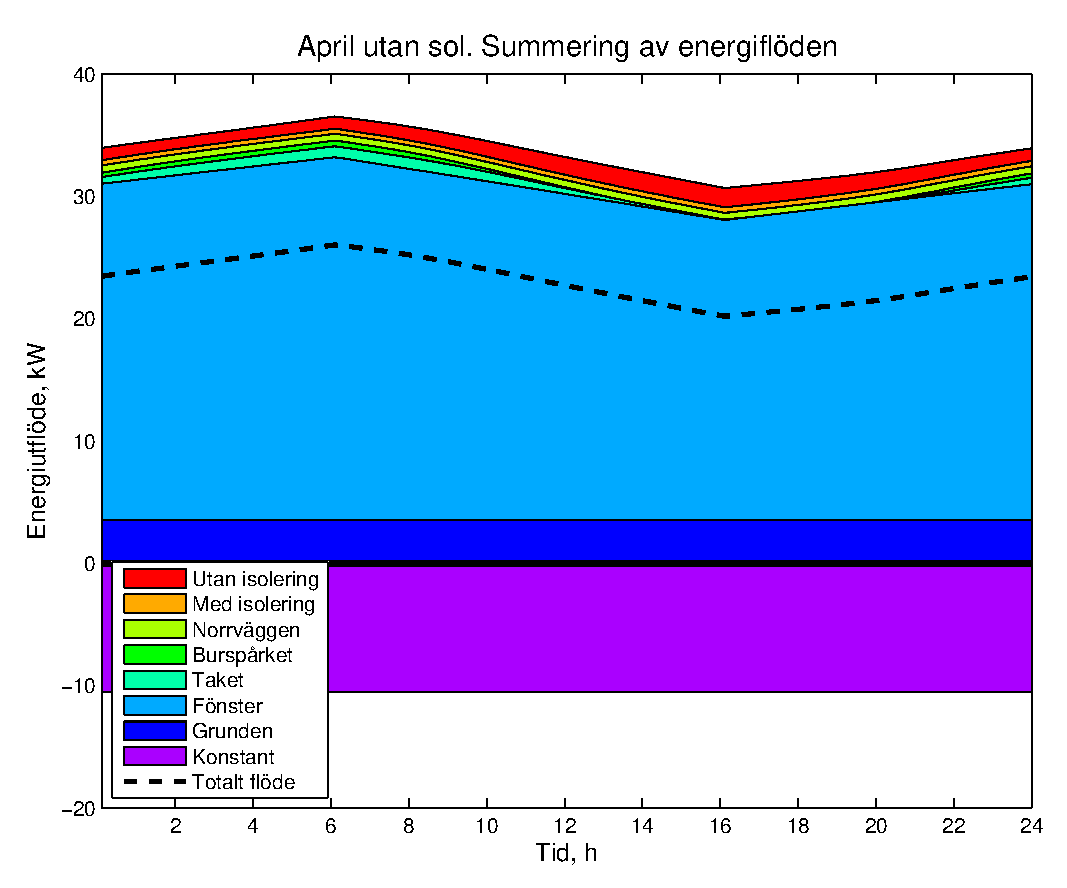
\includegraphics[width=0.5\textwidth]{images/aprnosun_sum.eps}
}
\subfloat[\label{fig:sum_aprsun} Aprildygn med solig dag]{
	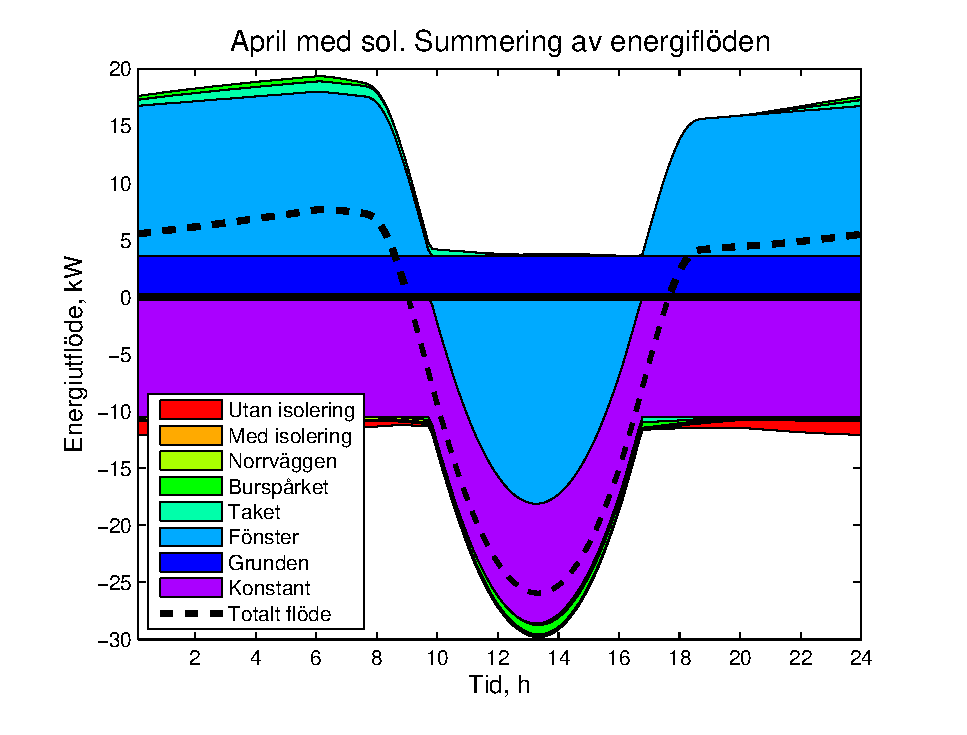
\includegraphics[width=0.5\textwidth]{images/aprsun_sum.eps}
}

\subfloat[\label{fig:sum_decnosun} Molnigt decemberdygn]{
	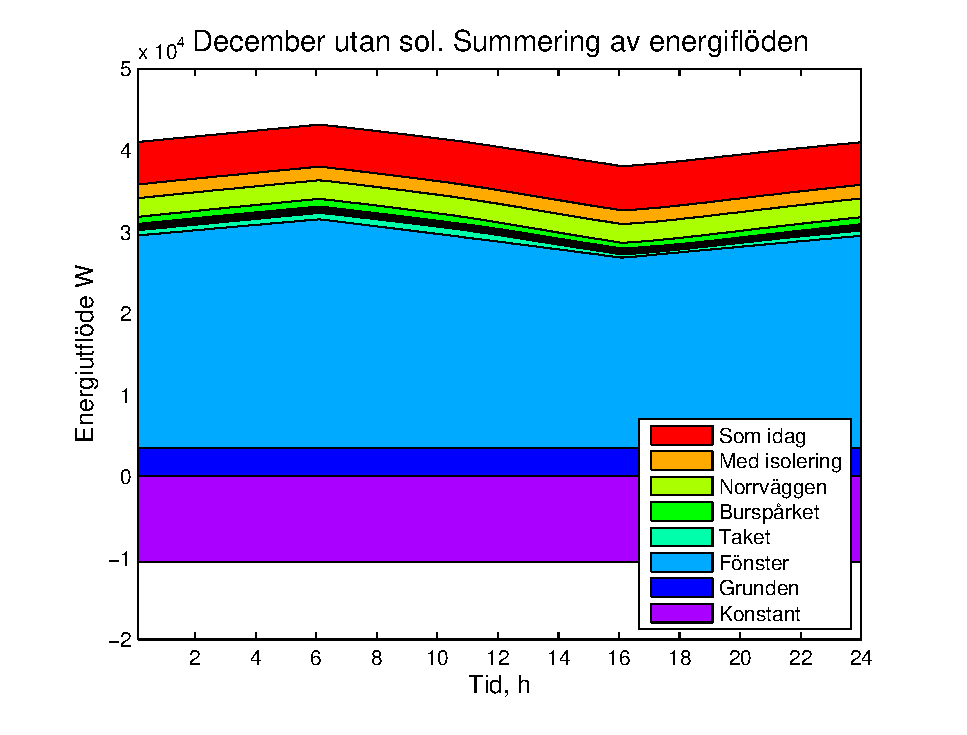
\includegraphics[width=0.5\textwidth]{images/decnosun_sum.eps}
}
\subfloat[\label{fig:sum_decsun} Decemberdygn med solig dag]{
	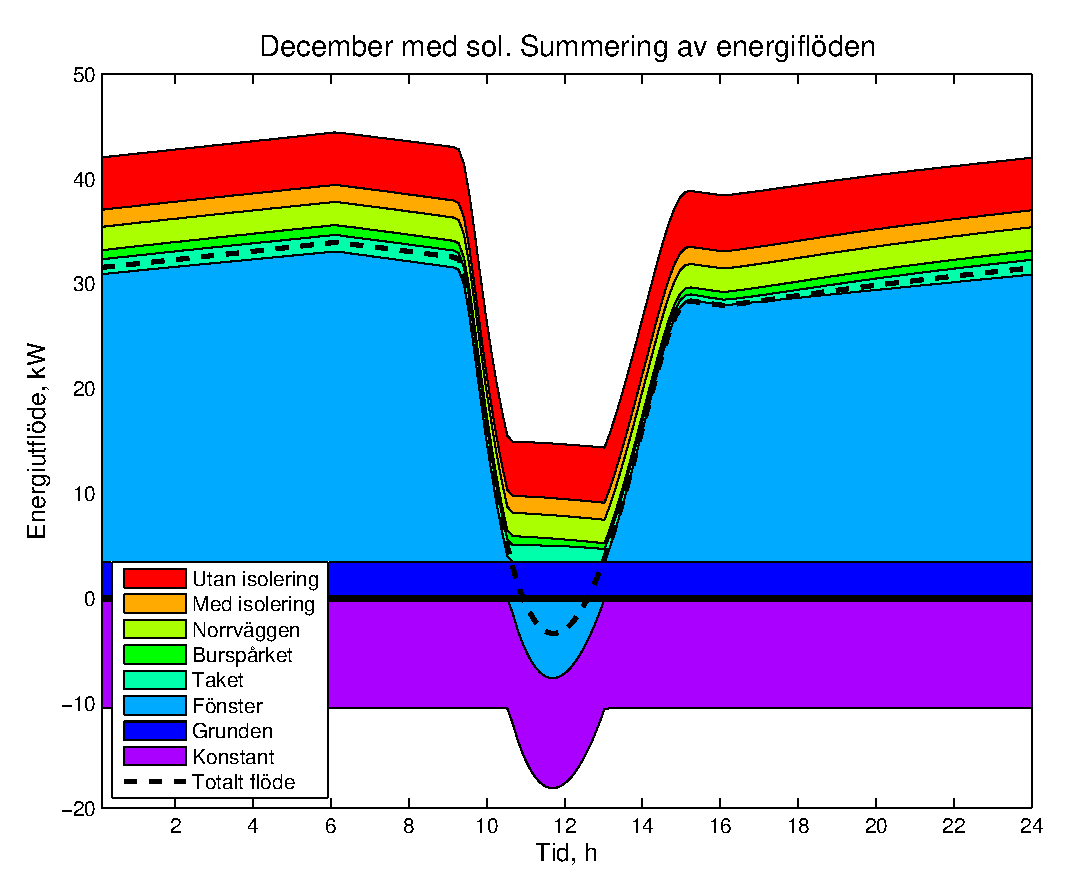
\includegraphics[width=0.5\textwidth]{images/decsun_sum.eps}
}

\caption{\label{fig:energyflow_sum} Totala energiflöden genom bygganden, där utflöden
 betecknas positivt, och inflöden negativt. Den steckade linjen markerar summering av 
 positiva och negativa energiflöden. Den heldragna, något bredare linjen är gränsen mellan in- och utflöden.}
\end{figure}

Det mest framträdande i bilderna är solens påverkan. Den andra är att fönstren läcker väldigt 
mycket energi. Under en solig aprildag, är det genom fönstren som den mesta energin 
kommer in när solen skiner och samtidigt som fönstren är den största energitjuven under 
resten av dygnet. Vi ser också att det under april knappast lönar sig att ha tilläggsisolerat syd-
 och västfasaderna, det gör det däremot i december. Fönstren är dock den enskilt största 
 källan till energiläckage.

Vid vind fås ytterligare energiförluster. Med en vindmätare mäts de enkelt i varje ögonblick och 
energiförlusten beräknas enligt avsnitt \ref{sec:leakagewall} och adderas till befintligt energiflöde. I figur \ref{fig:windenergyloss} ser vi att vi vid $\unit[20]{m/s}$ och utomhustemperatur $\unit[0]{^\circ C}$, det vill säga en temperaturdifferens på $\unit[20]{^\circ C}$ mellan inom och utomhus får vi som mest en energiförlust på $\unit[2]{kW}$. Detta kan jämföras med utstrålning genom fönster ofta är över $\unit[20]{kW}$.